\documentclass[11pt, letterpaper]{article}
\usepackage{graphicx}
\usepackage{placeins}
\usepackage[margin=1in]{geometry}
\usepackage{adjustbox}
\usepackage{float}
\usepackage{cite}
\usepackage{longtable}
\usepackage{booktabs}

\title{Comparing performance and viability of PQC on different architectures}
\author{Olivier Gillot}

\begin{document}
\maketitle

\begin{abstract}
With Q-day getting nearer, the great PQC transition has started and the US, UK and EU governments are all taking steps to move the internet towards a Quantum-resistant encrypted world. In this paper, we tested the NIST-approved algorithms FIPS 203 (ML-KEM), FIPS 204 (ML-DSA) and FIPS 205 (SLH-DSA), in Key-Generation, Signing and Verifying methods for the time and energy metrics across a range of IoT-style devices, from the 32-bit Raspberry Pi 1 and Zero to the 64-bit Raspberry Pi 4. Using a FNB58 power reader, we found that ML-KEM and ML-DSA delivered on the promise of being as energy and speed efficient as traditional Elliptic Curves, but that it would be inadvisable to run any SLH-DSA signature on constrained hardware, particularly with a 32-bit architecture, where energy costs for SLH-DSA signing were found to be 243\% higher than on equivalent 64-bit hardware.
\end{abstract}

\section{Introduction}

This section introduces the aim of the paper and the technological and security landscape which lead to the experiment.

Anyone old enough to have seen Jurassic Park on its first theatrical release will easily remember the days when the internet was a wild place, with no moderation whatsoever, and where encryption was uncommon by default. Anyone could easily access and read all our communications, and there were no limits to the abuses of power that this lack of privacy entailed. However, brilliant academics had a solution: encryption. Following the footsteps of giants such as Rivest, Shamir and Adleman (RSA public key encryption), Diffie and Hellman (ECDH key exchange), Daemen and Rijmen (AES symmetric encryption), the industry, spearheaded by Google and its ubiquitous Chrome browser, took the decision to mark any non-encrypted website as insecure, which led to a global implementation of privacy and encryption to much of the internet: currently, between 95 and 99 percent of web navigation in Chrome is protected and inaccessible to eavesdropping thanks to the HTTPS protocol and the TLS standards. \cite{thompson2025https}
This shift towards a private and secure internet has thankfully resisted some governments push for back doors \cite{kleinman2025apple}, however, the encryption methods which have been around for decades are now under a new technological threat: Quantum Computing. \cite{buchanan2025quantum}
By leveraging new progress in experimental physics, scientists have proven that a new type of computer, the Quantum Computer, is so efficient at factorising large numbers that it is estimated that in the near future, using Shor’s \cite{shor1994algorithms} algorithm, public key encryption could be broken. Currently it only exists at small scale, but there is a race between state-actors to be able to develop one at a large scale, and the date for a fully usable Quantum computer keeps getting closer. \cite{buchanan2026qday}

And while AES-256 symmetric encryption seems safe for now \cite{buchanan2023aes}, since the public key encryption is used precisely to share symmetric keys, we can see that breaking RSA or ECDH would reveal the private keys, therefore effectively breaking the encryption. And encryption works in such a way that it is either entirely safe or completely broken. The “safe-enough-for-now" is nonsensical: anything that was deemed safe in 1980 is now commonly trivial to decrypt and with “Harvest-now, decrypt-later", we can easily imagine a future where all our currently encrypted conversations could be decrypted and explored by an advanced AI monitored by malicious agents or rogue-state actors. \cite{enisa2021current}
The answer to this is Post Quantum Cryptography (PQC): a series of algorithms that efficiently protects encryption against hypothetical attacks led by large Quantum computers.

Of course scientists and governments have been working at solving the challenge. In Europe, the NCSC in Britain \cite{ncsc2025migrating} and the European Commission \cite{ec2025pqc} have laid the path to the PQC transition, while the American government agency NIST has launched a vast project to find, select and implement quantum-computing resistant algorithms. At the time of writing, three candidates have been officialised: ML-KEM (Kyber), ML-DSA (CRYSTALS-Dilithium) and SLH-DSA (SPHINCS+) \cite{csrc2024post}. 
Considering the importance of the shift to come, there is a need in literature for an exploration on the strength and viability of these algorithms. Building on the works of J. Patterson et al.\cite{patterson2025energy} and Turino et al.\cite{turino2025pqc}, I decided to expand their ideas by including signatures and verification beyond the key generation algorithms and to test a variety of machines, including very low powered ones, such as a Raspberry Pi first generation or a Pi Zero, by testing them both on speed and on power consumption.
The implementation of the NIST-approved algorithms in OpenSSL 3.5 in April 2025 \cite{openssl2025pqc} gives us a great opportunity: it is indeed possible to run OpenSSL on pretty much any device (although installing it does take a few hours on the smaller ones), and we can now compare efficiently both the traditional and PQC algorithms on the same machine without advanced implementation.
Hence, by testing variants of the three NIST approved-algorithms in both power consumption and speed against classic cryptography, we managed to have a larger picture of the viability (or lack-of!) of the PQC on a variety of constrained devices. To conduct the tests, I used a range of Raspberry Pis (32-bits and 64-bits) alongside some ARM and x86 laptops to cover as many architectures as were available to me.


\section{Literature Review}
\subsection{Context}
Post-Quantum Cryptography is a very current topic, which has huge implications for both governments and private companies everywhere. There is abundant literature on the topic, but for contextual texts, I would refer to Shor’s foundational paper \cite{shor1994algorithms} which described in 1994 the theoretical basis on which Quantum computers may be able to break the traditional RSA and Elliptic curve algorithms. The Q-day, this day where quantum computing becomes a reality beyond prototyping, is getting nearer, as underlined by Prof. Buchanan in a recent article \cite{buchanan2026qday}, in which he informs us of the recent advances in qubit research, by Webster \cite{webster2026pinnacle} and Gidney \cite{gidney2025factor}.
It is not only academics who are moving fast on this. The US agency NIST has been proactive in considering the shift towards PQC and has selected three algorithms (with another algorithm, HQC, pending) for standardisation, alongside a deadline for migration for all American Federal systems by 2035. \cite{moody2024transition,moody2025roadahead} In Britain, the NCSC has recommended that a target of 2028 be in place for initial migration, 2031 for complete migration for highest priority services and 2035 for complete migration on all systems, services and products \cite{ncsc2025migrating,national2025timelines}. The European Commission has also been proactive on the matter, recommending that all Member States initiate a PQC transition strategy by 2026, that high-risk use cases should be transitioned as soon as possible, no later than 2030 and that by 2035 the transition should be completed as far as possible. \cite{ec2025pqc}
\subsection{Foundational work}
The main idea behind my paper is based on the ‘Energy Consumption Framework and Analysis of Post-Quantum Key-Generation on Embedded Devices’ by Patterson \cite{patterson2025energy} After reading it (and enjoying it!), I decided to build on his idea, to measure PQC energy consumption on a Raspberry Pi device using OpenSSL 3.5 to run the algorithms, and expand on his work by adding a larger variety of devices and by adding signing and verifying alongside key-generation. The reason behind this being that a Raspberry Pi 5 has become quite a capable machine and no longer represents low-power embedded devices as well as an early Raspberry Pi (1 or 2) or a Pi Zero might do. And key-generation alone is not the most significant algorithm for hardware limitation, as the signing results will demonstrate. Finally, and following the example of C.Turino in his paper ‘PQC-LEO: An Evaluation Framework for Post-Quantum Cryptographic Algorithms’ \cite{turino2025pqc}, I decided also to test algorithms beyond ML-KEM, with signature algorithms ML-DSA and SLH-DSA to explore the actual limitations of smaller hardware, by taking inspiration from his framework –if not quite matching its scale.
\subsection{Related PQC benchmarking literature}
Tasopoulos et al. \cite{tasopoulos2023energy} measured PQ TLS 1.3 energy consumption on a single STM Nucleo embedded board using WolfSSL. Whilst they did indeed manage to have much more precise readings than me thanks to a high-end oscilloscope -compared to my simpler FNB58- and achieved the readings for the full TLS 1.3 exchange, which was attempted but left as future works, they also tested only one machine (Single STM Nucleo Cortex-M4) with a custom embedded WolfSSL script. My solution explored multiple, more constrained hardware (down to a Pi at 700MHz), with the stock OpenSSL 3.5, and is reproducible by anyone with a Unix machine. Their work was also published pre-standardisation and therefore is not using the current FIPS names. They found that “SPHINCS+ needs tremendous amounts of energy and time just for a single handshake.” which matches my own findings for very constrained devices (32 bits Pi 1, 2 and Zero) despite the completely different methodology.

Paquin et al. \cite{paquin2020benchmarking} benchmarked PQC algorithms in TLS under emulated network conditions, focusing on how packet loss and latency affect performance. They took a completely different approach than mine, by focusing on network constraint rather than raw compute power. They based their research on extremely capable cloud hardware (Azure D64s with 64 vCPUs) and an emulated network. They do check the full TLS exchange, pre-standardisation, with a custom OQS-OpenSSL fork predating the native PQC support in OpenSSL 3.5. Both their solution and mine are complementary: what happens on bad hardware, or what happens on a bad network!

Schöffel et al. \cite{schoffel2021energy} evaluated energy costs of PQC KEMs in TLS on a low-power IoT Cortex-M4 device, showing accelerators are not necessary for feasible deployment. The authors used a more genuinely “IoT” device than the ones I had access to: a Cortex-M4 at 64MHz with 256KB RAM is seriously more constrained than even my Pi 1 or my Pi Zero. This is a single purpose-built IoT chip, whilst I covered a range of more general-purpose devices. They only focused on KEM algorithms, whilst my solution incorporates signing with SLH-DSA. Their findings do match mine regarding the KEMs, and they state that: “proving that the usage of post-quantum KEMs is already feasible today in terms of energy demand and latency for low-power IoT with state-of-the-art hardware” which mirrors my findings, regarding ML-KEM algorithms (SLH-DSA presenting, however, a different picture on constrained hardware.)

S Sarıbaş, S Tonyalı \cite{saribacs2022performance}, Bozhko et al. \cite{bozhko2023performance} measured TLS 1.3 handshake performance (packet overhead and delay) of pre-standardisation PQC algorithms on resource-constrained devices over Ethernet, BLE and WiFi networks. In Sarıbaş’s paper, the authors focussed on a different metric to the ones I have considered, the packets across an ethernet network. Whilst Bozhko et al. took a similar approach over a wireless network (BLE and WiFi) They used Raspberry Pis 4 to communicate over a switch network, using pre-standardisation algorithms, captured the data with Wireshark and drew their conclusions without measuring power. This is complementary to my work, which only focussed on local hardware energy usage and speed testing. But while I do test a Raspberry Pi 4 in my machines, it is actually a rather capable machine and not very representative of constrained hardware. However, network and packet capture would fall neatly into a future expansion of my work.

Roma et al. \cite{roma2021energy} analysed the energy consumption of all NIST Round 2 PQC candidates on a single Intel i7 using software-based power measurement via PAPI/RAPL. Interestingly, they chose a solution I decided not to use. During my initial testing, I found that software measurements of power draw had some fundamental flaws, it is imprecise and always only an estimate. This is precisely why I purchased a FNB58 and took all my measurements manually to be as close as possible to real, easily repeatable readings.  Whilst they did check many more algorithms than me, I focussed my efforts on the NIST standard ones and on comparing them to traditional methods. Hence our papers are related in topic, but differ in scope, as they acknowledge: “which make it difficult to make a correlation between the energy measurements obtained in this work to the energy consumption expected on a low-end embedded processor.” This is where my work completes theirs by bringing in low-end processors and physical readings.

In a recent paper (January 2026), Algar-Fernandez et al. \cite{algar2026benchmarking} benchmarked timing performance of standardised and research-stage PQC primitives across two commodity Windows CPUs using a Python TCP testbed without energy measurements. They assessed the different methods, key-generation, signing and verifying. They did not use OpenSSL like I did, lowering the ease of reproducibility, and acknowledge themselves that: “This study emphasizes execution time and includes size-related indicators where available. It does not provide a systematic evaluation of additional deployment-relevant metrics such as memory consumption, energy usage, side-channel resistance, or formal constant-time validation.” and that “they do not capture the full diversity of deployment environments (e.g., servers with different microarchitectures, Linux-based infrastructure, mobile devices, microcontrollers, and specialized accelerators). Results may therefore differ on other hardware/software stacks”. And different hardware/software stacks are precisely what I did, with a Linux/macOS and ARM architectures (alongside an AMD and an Intel x86 the same way they did.)

\section{Implementation}
\subsection{Hardware}
\subsubsection{The Pis}
Considering my literature review, I decided to focus my main efforts on Raspberry Pi from early generations and smaller processors. The fact that I already owned 4 of them from past projects made this decision rather simple, I only had to procure a Raspberry Pi 2 v1.1, Raspberry Pi 2 v1.2 (whilst very similar, the second one is actually 64-bits enabled, leading to an interesting test of the practical difference between 32 and 64-bits architecture on ARM devices) and a Raspberry Pi 3 (Model A+).

This gave me a lineup of 7 different ARM machines ranging from 700MHz single-core and 512MB of memory for the Raspberry Pi 1 to the 1.5GHz quad-core Pi 4 with 8GB of LPDDR4 memory, a very capable machine (which was used as a desktop replacement, a retro-gaming console, a webserver and a smart tv, at times.)

\begin{table}[h]
\centering
\caption{Raspberry Pi Hardware Specifications}
\label{tab:raspberry-pi-specs}
\begin{adjustbox}{max width=\textwidth}
\begin{tabular}{|l|l|l|l|l|}
\hline
\textbf{Model} & \textbf{OS} & \textbf{CPU} & \textbf{Memory} & \textbf{Arch} \\
\hline
Raspberry Pi 1 Model B & Debian Bookworm & 700MHz single-core ARM1176 & 512MB LPDDR2 & 32-bit (ARM) \\
\hline
Raspberry Pi 2 Model B v1.1 & Debian Bookworm & 900MHz quad-core ARM Cortex-A7 (ARMv7) & 1GB SDRAM (450MHz) & 32-bit (ARM) \\
\hline
Raspberry Pi 2 Model B v1.2 & Debian Bookworm & 900MHz quad-core ARM Cortex-A53 (ARMv8) & 1GB SDRAM (450MHz) & 64-bit (ARM) \\
\hline
Raspberry Pi Zero WH & Debian Bookworm & 1GHz single-core ARM1176 & 512MB LPDDR2 & 32-bit (ARM) \\
\hline
Raspberry Pi Zero 2 WH & Debian Bookworm & 1GHz quad-core ARM Cortex-A53 & 512MB LPDDR2 & 64-bit (ARM) \\
\hline
Raspberry Pi 3A+ & Debian Bookworm & 1.4GHz quad-core ARM Cortex-A53 & 512MB LPDDR2 & 64-bit (ARM) \\
\hline
Raspberry Pi 4 & Debian Bookworm & 1.5GHz quad-core Cortex-A72 & 8GB LPDDR4 & 64-bit (ARM) \\
\hline
\end{tabular}
\end{adjustbox}
\end{table}

The figure 1 presents all the Raspberry Pis and the FNB58 used in my experiments.

\begin{figure}[h]
    \centering
    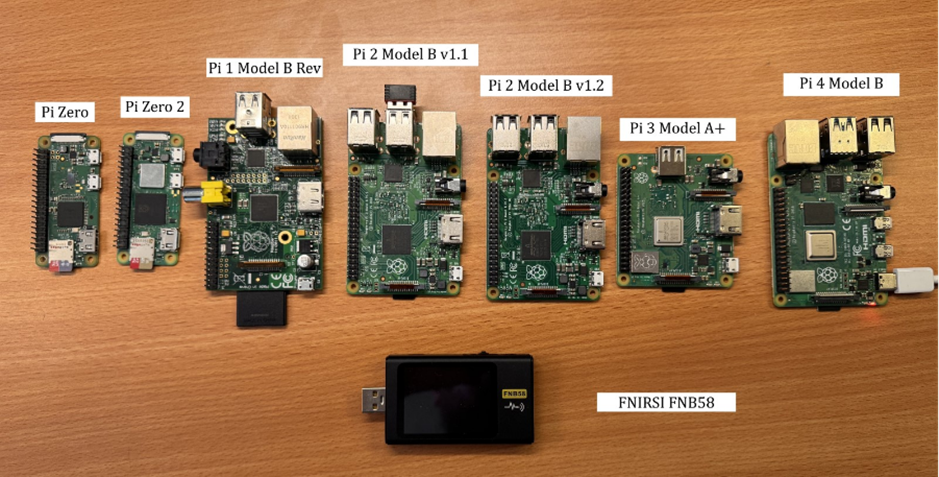
\includegraphics[width=1\linewidth]{lab_setup.png}
    \caption{Raspberry Pi lineup and FNB58}
    \label{fig:labsetup}
\end{figure}

\subsubsection{The FNIRSI FNB58}
After researching it on specialised websites \cite{elektor2023fnb58}, I found that the FNIRSI FNB58 would be the perfect choice for my tests. Its simplicity of use, accurate readings and reasonable price made it the perfect tool.

\begin{figure}[H]
    \centering
    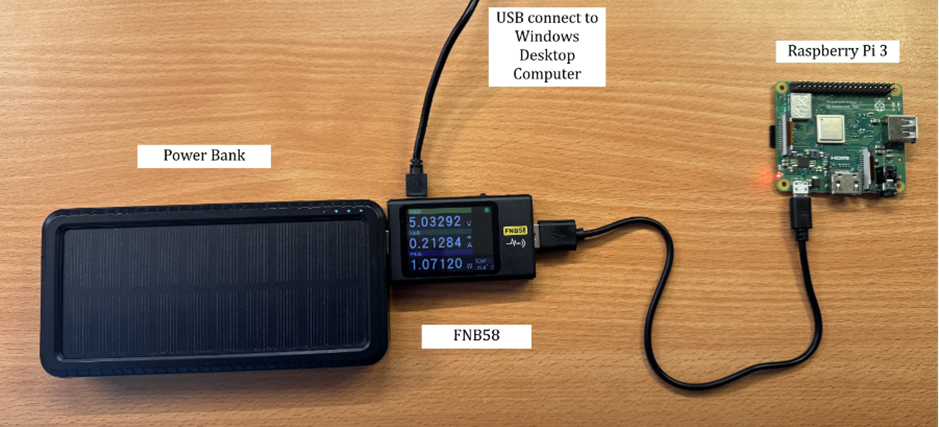
\includegraphics[width=1\linewidth]{fnb58.png}
    \caption{FNB58 in operation}
    \label{fig:fnb58}
\end{figure}

To operate it, I needed to connect it between a power bank for 5V (up to 2.1Amp) power delivery and a micro-usb cable connected to the Raspberry Pi to power it and record the power variations. The figure 2 presents the FNB58 in operation.

\subsubsection{Laptops and Desktop machines}
I also used my three laptops, an Ubuntu Thinkpad T480s Intel from 2017, a MacBookAir M1 (ARM) from 2020 and a 2024 Thinkpad P14s Gen5 AMD. It allowed me to have three more different architectures. Due to the complexity of isolating power readings for the OpenSSL load and the unreliability of software estimations, I only ran timed tests on these.

\begin{table}[h]
\centering
\caption{Laptop Hardware Specifications}
\label{tab:laptop-specs}
\begin{adjustbox}{max width=\textwidth}
\begin{tabular}{|l|l|l|l|}
\hline
 & \textbf{Thinkpad T480s Intel} & \textbf{MacBookAir M1} & \textbf{Thinkpad P14s Gen5 AMD} \\
\hline
\textbf{OS} & Ubuntu 25.10 & macOS Tahoe 26.3 & Ubuntu 24.04 \\
\hline
\textbf{CPU} & Intel Core i7-8550U & Apple M1 (ARM) & AMD Ryzen 5 PRO 8640HS \\
\hline
\textbf{Memory} & 40 GB DDR4 & 8 GB LPDDR4X & 16 GB DDR5 \\
\hline
\textbf{Arch} & 64-bit (x86-64 Intel) & 64-bit (ARM-M1) & 64-bit (x86-64 AMD) \\
\hline
\end{tabular}
\end{adjustbox}
\end{table}

My Windows 11 AMD Desktop machine was used to coordinate and control all the different machines via WSL Ubuntu and SSH, and to gather the FNB58 data via micro-usb cable on their proprietary windows-only software.

\subsection{Software}
\subsubsection{OSes}
Each of the Raspberry pi machines was freshly imaged using the Raspberry Pi Imager utility to flash a lightweight desktop-free Debian Bookworm distro on a micro-SD card (and SD-card for the Raspberry Pi 1). This ensured that the very minimum other processes would be interfering with our power reading collection.

Both Thinkpad Laptops are running Ubuntu and the MacBookAir runs MacOS Tahoe. Having all machines running on Unix allows us to run the same programs without having to have multiple versions. Since I am not running power readings, I did not need fresh installs on these, I simply turned off all irrelevant programs and processes when I ran the speed tests.

\subsubsection{OpenSSL 3.5}
Fundamental to this paper, the stock version of OpenSSL 3.5 includes all the PQC algorithms central to our testing (ML-KEM, ML-DSA, SLH-DSA) \cite{openssl2025pqc}. By being able to run exactly the same program (OpenSSL) on a variety of algorithms on a variety of machines ensures we get fair readings, depending only on variations of hardware instead of different software implementations.

Installing OpenSSL has proven to be a rather lengthy process for the weaker Pis. It took several hours to install it on the Raspberry Pi 1 and the Pi Zero, however, as our results stand to show, it is doable. Whilst OpenSSL ships as standard on Linux distributions and MacOS, I needed the 3.5 version which was not included in any of the distros used, therefore requiring a manual build from source for all the machines. All the command lines used are to be found in the appendix and on the GitHub of this project.

\subsubsection{USB-meter and .cfn format conversion}
To record the power readings, another fundamental point of the project, I had to use the proprietary program, the USB-meter v0.7, found on the FNIRSI website. \cite{fnirsi2025software} It allowed me to view and record the PBUS (watts) data, the most important for my data collection, as seen in the figure 3:

\begin{figure}[h]
    \centering
    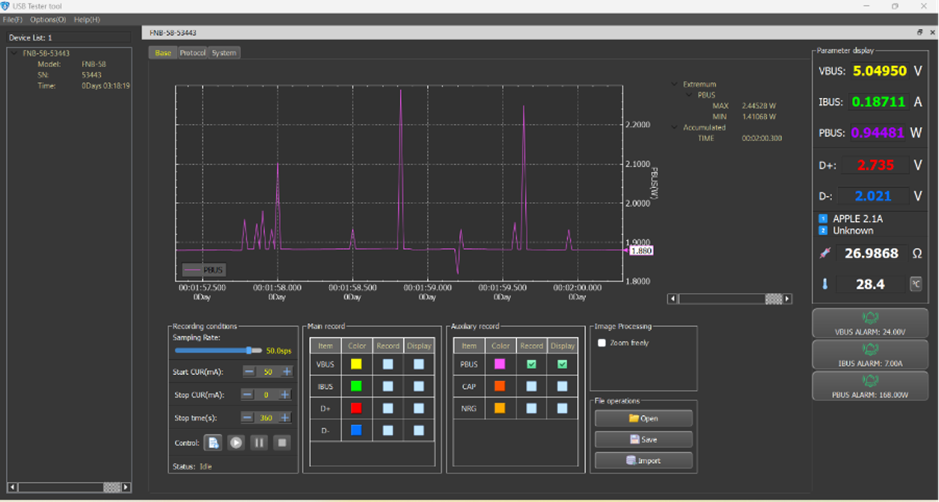
\includegraphics[width=1\linewidth]{usb_meter.png}
    \caption{USB-meter in operation}
    \label{fig:usb-meter}
\end{figure}

The program shipped with the FNB58 unfortunately only saves data with a proprietary format, .cfn. To circumvent the problem, my thanks to Andrey Volkov who created a utility to turn these files into .csv files. \cite{volkov2025usbmeter}

\subsection{Measurement procedures and data collection}
\subsubsection{Power readings}
Once all the hardware has been procured and the software installed, the first step was to gather accurate power readings for each of the seven Raspberry Pi.

The same steps were repeated for every machine. Firstly, after a few minutes of warm-up, I would connect to the Pi via SSH to launch the commands. I would always check that no processes were running in the background, and then from the USB-meter utility, would record a 5 minutes baseline at 50 samples per seconds PBUS for idle. I would then save the file, as a .cfn file. Then, with usb-meter-utils, I would simply convert the .cfn file into a usable .csv file. Then it is simple to average the PBUS column values to get an average baseline idle power reading.

Then I would use pqc\_benchmark.py (described below) to select which method/algorithm to run, select a very large number of iterations to make sure it does not finish before the recording is done, and record an approximately 30 seconds interval whilst the program is on-load. This relatively small interval (which collected circa 6000 samples at 50sps) was due to time constraints: having to run 32 algorithms per machine, for 7 machines led to 224 samples to take. Then I would proceed the same way than for the baseline to collect the average of on-load power reading. All the .cfn and .csv files are available for review on the GitHub.
Tables summing up the power readings are available in the Appendix.

\subsubsection{Python wrappers programs}

In order to make the testing practical at scale, I created Python programs as wrappers for the OpenSSL operations. Both programs (pqc\_benchmark.py and pqc\_benchmark\_automated.py) are available for review in the GitHub of the project.

They simply compile all the OpenSSL commands, including creating keys, creating certificates, creating a message to be signed and/or verified, for every algorithm tested in a convenient program which lets the user select the number of iterations, and offers the possibility of an automated option for fast benchmarking. The power values may be optionally added, and all results are given a csv file.

Anyone with OpenSSL 3.5 enabled (complete steps for building it are in the GitHub of the project) running on a Unix machine can run both these programs. Please note that both programs are needed to run the automated benchmark, and that multiple files -keys, certificates, message to be signed and verified) are created in the process in sub-folder.

\subsubsection{Time metrics readings}

To get the time metrics, two options are available: a fast, automated test where the Python wrapper program only takes one variable, the number of iterations, and automatically runs every available algorithm (pqc\_benchmark\_automated.py) and puts them in a csv results file. This makes it ideal for testing of any Unix machine without power readings involved. The second option has more granularity, with a Python wrapper which lets the user select the method, the algorithm, and enter the power metrics to increment a csv results file.

\subsubsection{Running the tests}

During my data-collection, I ran every algorithm and method through the power metrics first, gathering the baselines and on-load power readings for every machine, method and algorithm for each of the seven Raspberry Pis
Then I ran each method with each algorithm on each machine, providing the gathered power-readings, on 100 iterations (except when the extreme slowness of SLH-DSA on slow devices forced me to only use 10) to gather my final results, samples of which are in the appendix and can be seen on the GitHub. Below is a table containing a small sample of the results, presenting the number of Joules needed per iteration.

\begin{table}[H]
\centering
\scriptsize
\caption{Key generation and signing, Joules per iteration across Raspberry Pi models}
\begin{tabular}{lccccccc}
\hline
 & pi1 & pizero & pi2 & pi2b & pizero2 & pi3 & pi4 \\
\hline

\multicolumn{8}{l}{\textbf{Keys}} \\

ecdh & 0.0483 & 0.0500 & 0.0380 & 0.0346 & 0.0382 & 0.0436 & 0.0319 \\
ml-kem-512 & 0.0519 & 0.0517 & 0.0398 & 0.0357 & 0.0388 & 0.0428 & 0.0345 \\
ml-dsa-44 & 0.0525 & 0.0519 & 0.0412 & 0.0361 & 0.0371 & 0.0444 & 0.0347 \\
slh-dsa-sha2-128f & 0.0601 & 0.0644 & 0.0503 & 0.0431 & 0.0464 & 0.0525 & 0.0407 \\
slh-dsa-sha2-128s & 0.7259 & 0.9182 & 0.7093 & 0.5521 & 0.6265 & 0.6304 & 0.4612 \\
slh-dsa-shake-192s & 2.0534 & 2.6092 & 2.2992 & 0.6654 & 0.7613 & 0.8485 & 0.6370 \\

\hline
\multicolumn{8}{l}{\textbf{Signing}} \\

ecdsa & 0.0254 & 0.0258 & 0.0206 & 0.0184 & 0.0192 & 0.0241 & 0.0197 \\
ml-dsa-44 & 0.0303 & 0.0320 & 0.0251 & 0.0218 & 0.0214 & 0.0284 & 0.0200 \\
slh-dsa-sha2-128f & 0.2757 & 0.3776 & 0.2711 & 0.2103 & 0.2359 & 0.2396 & 0.1730 \\
slh-dsa-sha2-128s & 5.1354 & 7.2222 & 5.1381 & 3.9943 & 4.5117 & 4.5984 & 3.2258 \\
slh-dsa-shake-192s & 18.7602 & 24.7630 & 19.6558 & 5.7308 & 6.5288 & 7.3749 & 5.4714 \\

\hline
\end{tabular}
\end{table}


\section{Evaluation}
Tables containing a sample of the tests results can be found in the Appendix.
\subsection{Viability of ML-KEM on constrained hardware compared to ECDH and X25519 for Key-Generation}

As the figure 4 shows, the ML-KEM (Kyber) FIPS 203 algorithm holds its ground when it comes to key-generation compared to the classic ECDH and X25519 elliptic curves. ML-KEM key generation remained within 2-12\% of ECDH and X25519 across all tested devices, with the single exception of ML-KEM-1024 on the Pi1 at 17\% overhead and the noticeably good results of Pizero 2 being actually marginally faster than ECDH. Schöffel et al. \cite{schoffel2021energy} specifically concluded: “the usage of post-quantum KEMs is already feasible today in terms of energy demand and latency for low-power IoT”, matching my findings that prove that the ML-KEM algorithms are a perfectly viable Quantum-safe replacement for the currently used but vulnerable elliptic curves.

It performed across the board, and even on very constrained 32-bits hardware such as the Pi 1 or the Pi Zero, making it perfectly plausible on a range of IoT devices.


\begin{figure}[H]
    \centering
    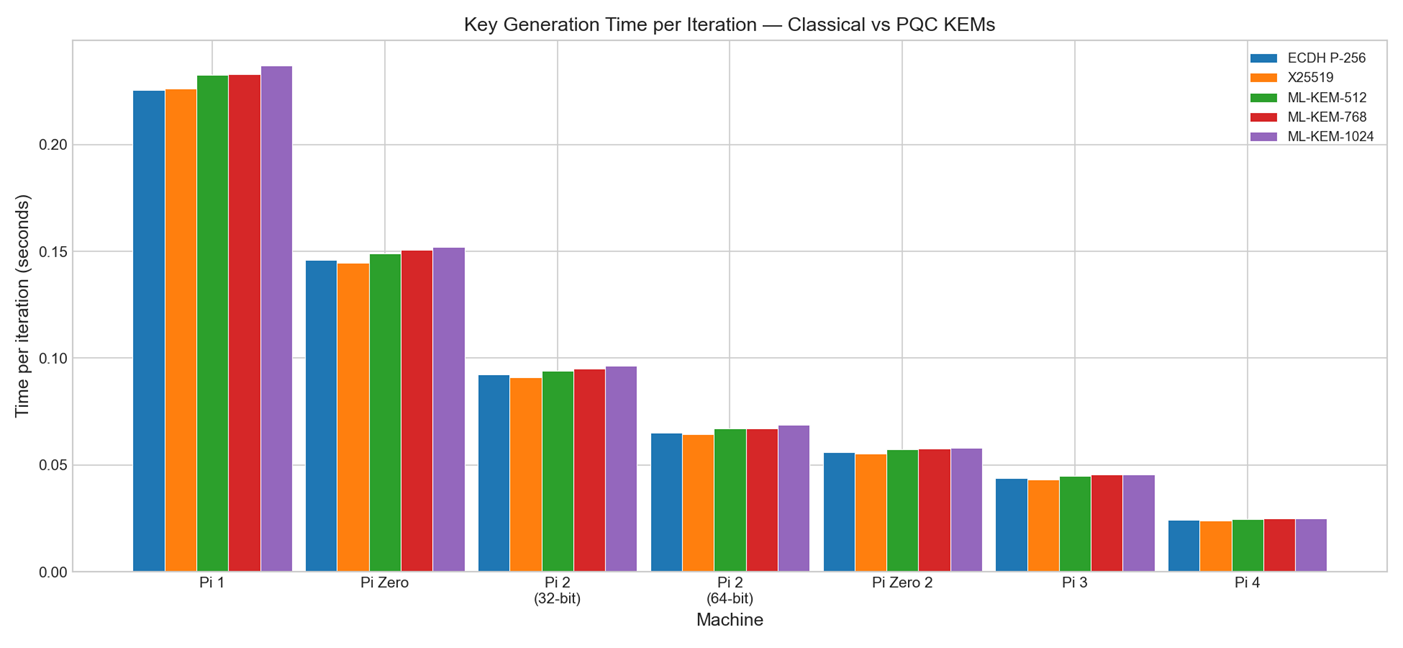
\includegraphics[width=1\linewidth]{key-gen-classical-vs-mlkem.png}
    \caption{ML-KEM on constrained hardware compared to ECDH and X25519}
    \label{fig:kengen-mlkem}
\end{figure}



\subsection{SLH-DSA vs ML-DSA performance and energy costs for Signatures}

\begin{figure}[H]
    \centering
    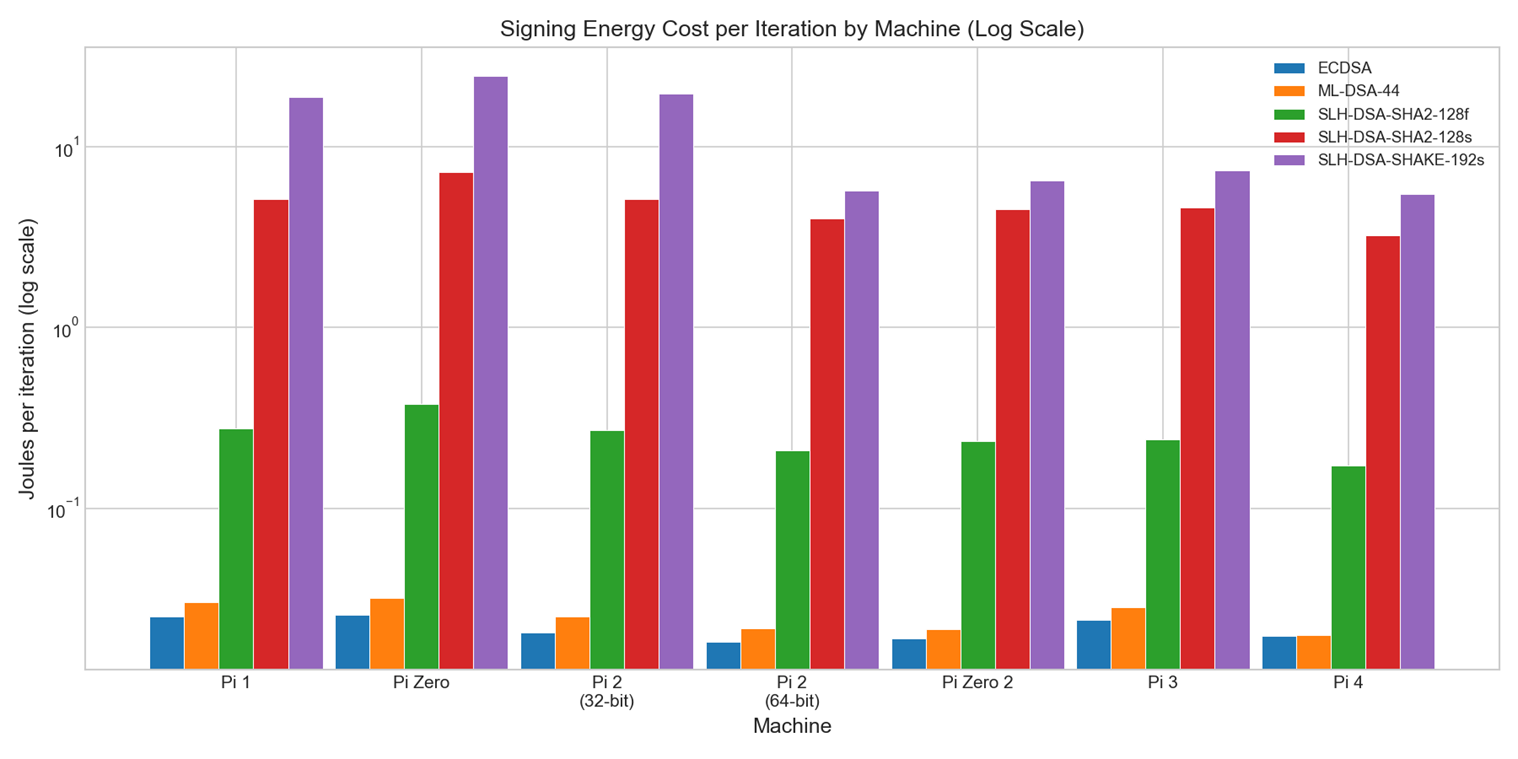
\includegraphics[width=1\linewidth]{signing-energy-log-scale.png}
    \caption{SLH-DSA vs ML-DSA performance}
    \label{fig:slh-vs-mldsa}
\end{figure}

As shown in the figure 5, whilst ML-DSA-44 (Dilithium) FIPS 204 got near the performance of ECDSA for Signing with a difference diminishing as the hardware gets more performant, from 19-24\% more energy used than ECDSA for the 32-bits devices to a 1.3\% on the Pi 4, it paints a very different picture for the SLH-DSA (SPHINCS+) FIPS 205 algorithms. I actually needed a logarithmic scale to be able to show how quickly the signature costs in Joules increase exponentially with these intentionally slow algorithms. They were designed to prioritise security conservatism through complex Merkle trees over performance, never to be used extensively and repeatedly on slow hardware as emphasised by Tasopoulos et al. “the NIST conservative security choice of SPHINCS+ as a Digital Signature (…) can only be used in a unilateral authentication since SPHINCS+ needs tremendous amounts of energy and time just for a single handshake” \cite{tasopoulos2023energy}, and our findings clearly match theirs and illustrate why. It is interesting to note that whilst it is possible to sign with SLH-DSA-SHAKE-192s on a Pi 1, it comes at such a cost that it may not be advisable, as the next section will show.

\subsection{Energy vs Speed: Key-Generation ML-KEM-768 and Signing SLH-DSA-SHAKE-192s}

In the figure 6, we look at the costs in Joules of 100 Key-Generation with ML-KEM 768 alongside how a very low power draw on the smaller CPU machines and 32-bits architecture nevertheless ends up consuming more Joules for Key-Generation. The reason is simple, whilst using a lot less power – the Pi 1 on-load delta draw is 0.212W, 6.6 times less than the Pi 4 1.41W delta draw for the same operation! – the speed of execution is the deciding factor, and the Pi 4, despite drawing more power, beats every other machine by simply being the fastest.

\begin{figure}
    \centering
    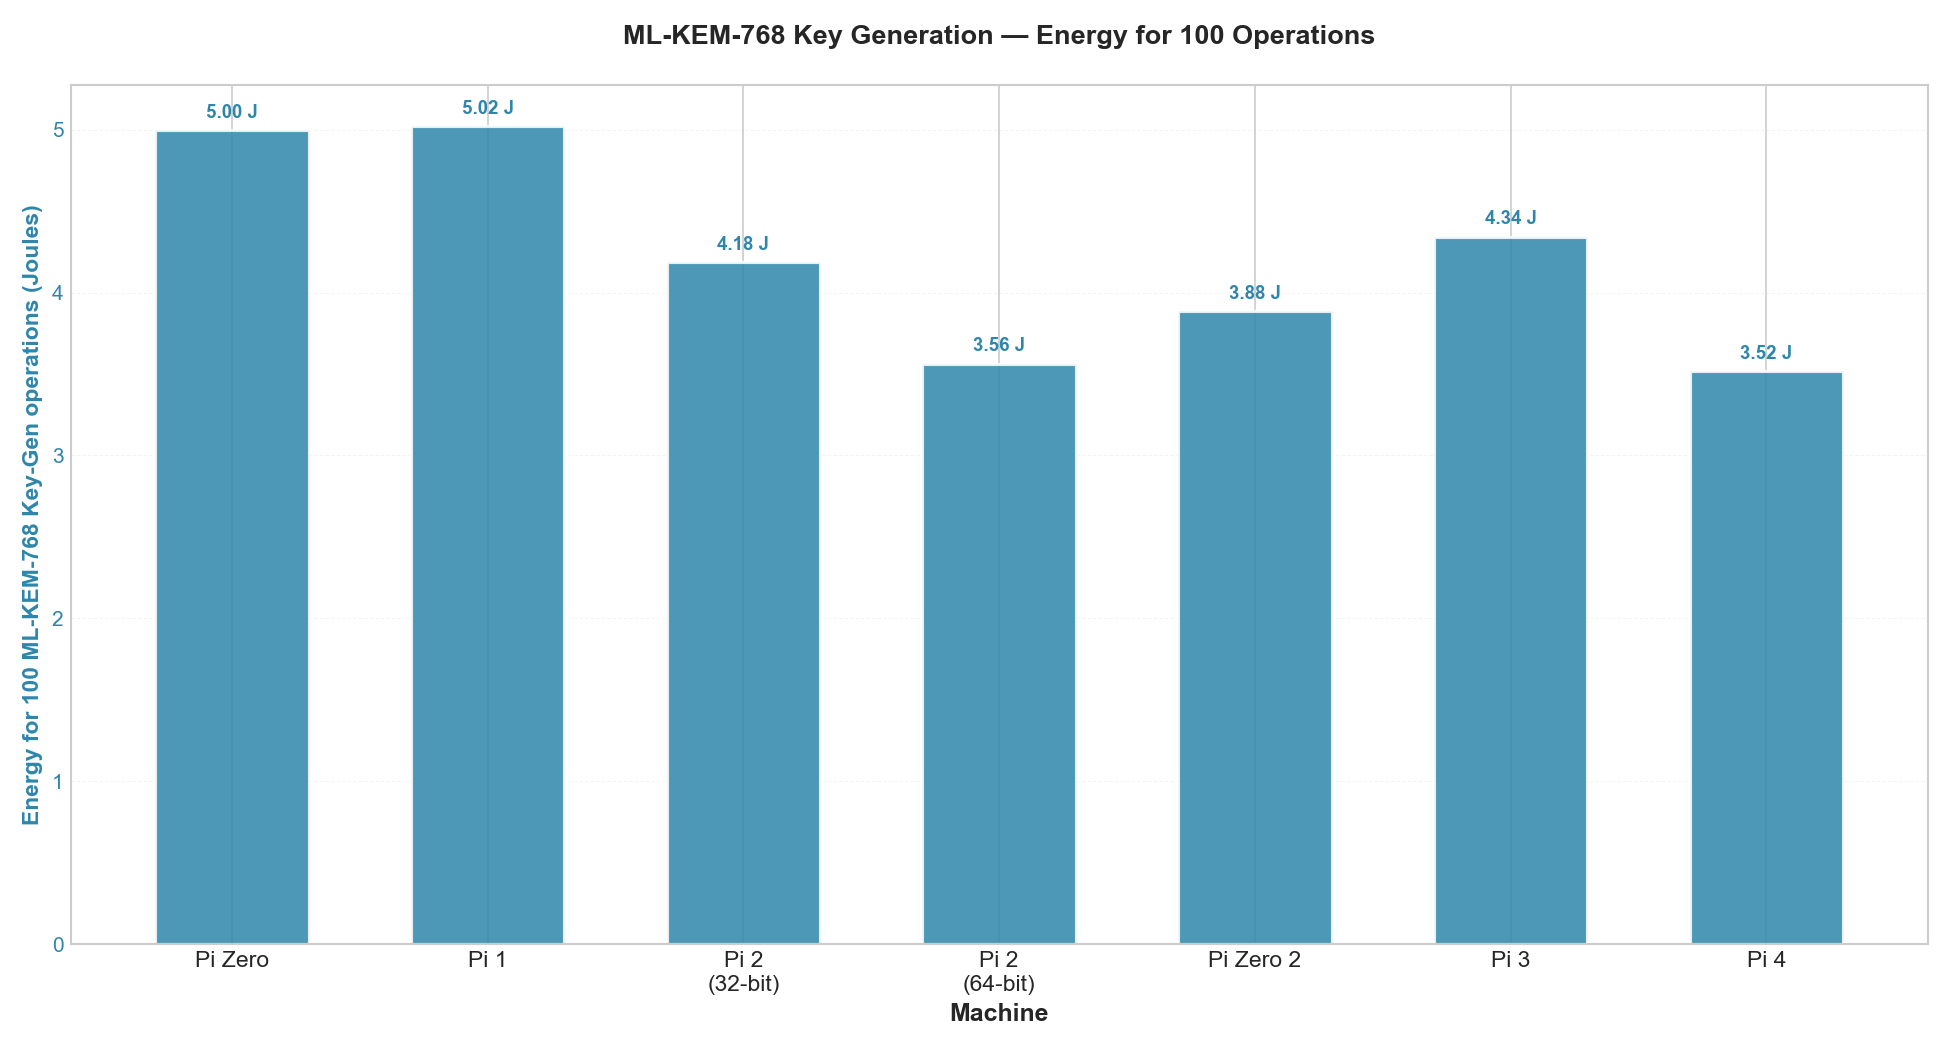
\includegraphics[width=1\linewidth]{mlkem_energy.png}
    \caption{ML-KEM-768 energy efficiency}
    \label{fig:mlkem-energy}
\end{figure}

The same logic applies to Signing with SLH-DSA-SHAKE-192s, but with an important difference. During key-generation, the Pi2 v1.2 64-bits performed 17\% better than its counterpart, the Pi2 v1.1 32-bits. With the much more demanding SLH-DSA-SHAKE-192s operation, the difference jumps to 243 percent increase on Joules needed for the 32-bits architecture. This finding clearly illustrates that whilst ML-KEM and Key-Generation is a perfectly viable option on slow devices, the costs and slowness of running SLH-DSA-SHAKE-192s Signatures on 32-bits devices makes it inadvisable.

\begin{figure}
    \centering
    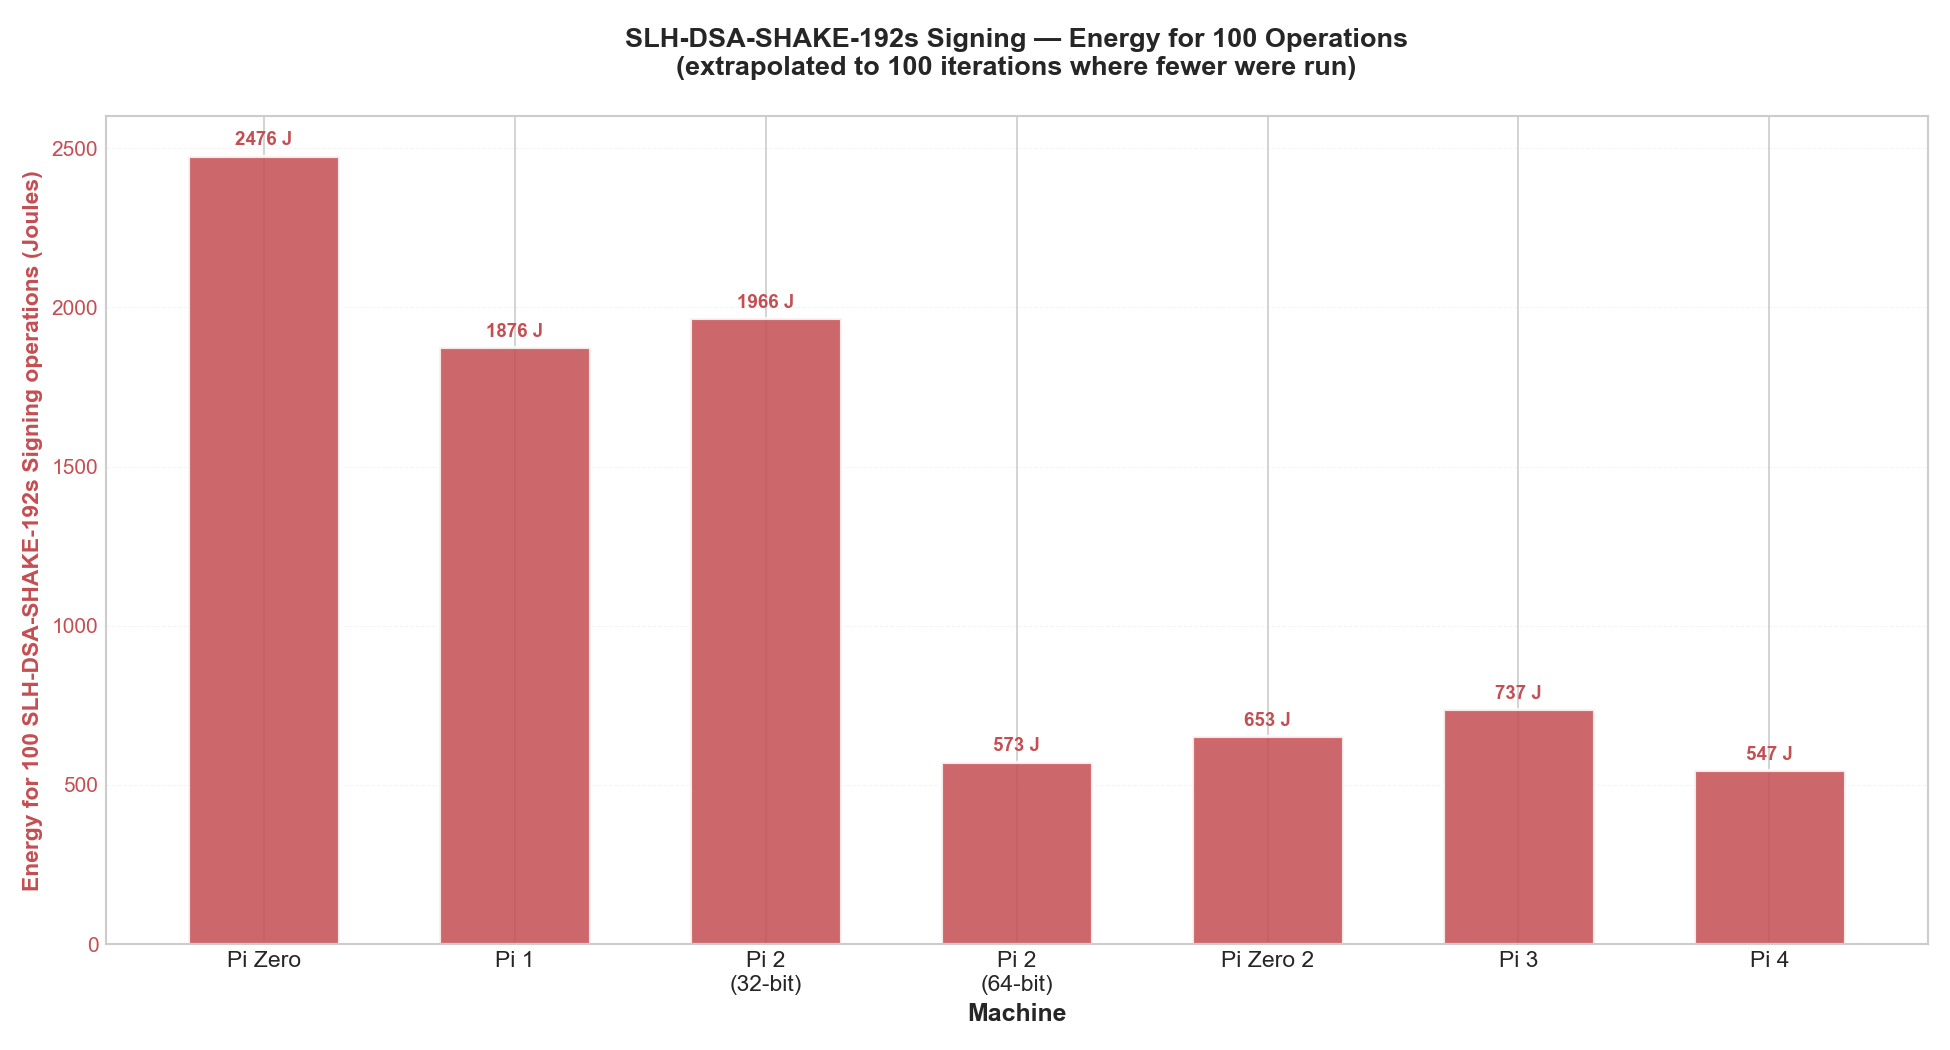
\includegraphics[width=1\linewidth]{slhsigningenergy.png}
    \caption{SLH-DSA-SHAKE-192s energy efficiency}
    \label{fig:slhsign}
\end{figure}

\subsection{Timing performance on x86 and ARM laptop vs Pi4}

A limitation in my testing was the inability to gather accurate power readings for the tests running on the different laptops that I had available. However, the timing metrics were easy to gather, and help serve as a point of reference against the Pis.
In the table below, we can note that the modern AMD Thinkpad is the fastest overall, only beaten by the M1 on SLH-DSA-SHAKE-192s signing, and whilst the M4 seems slower than the M1, a non-sense considering the huge difference in hardware, the anomaly may be explained by the use of a different OpenSSL build (namely, OpenSSL 3.6), and the verifying method was not included in the automated benchmarking. We can also notice that the Pi4 clearly holds its own respectably against much more capable machines on ML-KEM and ML-DSA, blurring the line between a laptop and what is perhaps inappropriately considered an embedded or IoT-class device.

\begin{table}[H]
\centering
\scriptsize
\caption{Cryptographic Performance — Time per Iteration (s) across laptops and Raspberry Pi 4. M4 data courtesy of Bill Buchanan.}
\begin{adjustbox}{max width=\textwidth}
\begin{tabular}{llccccc}
\hline
Algorithm & Operation & Pi 4 & MacBook Air M1 & ThinkPad Intel & ThinkPad AMD & MacBook Pro M4 \\
\hline

\multicolumn{7}{l}{\textbf{Key Generation}} \\

RSA-2048 & KeyGen & 0.3526 & 0.0576 & 0.0538 & 0.0408 & 0.0868 \\
ECDSA P-256 & KeyGen & 0.0247 & 0.0124 & 0.0104 & 0.0072 & 0.0333 \\
X25519 & KeyGen & 0.0239 & 0.0118 & 0.0111 & 0.0073 & 0.0328 \\
ECDH P-256 & KeyGen & 0.0243 & 0.0123 & 0.0114 & 0.0074 & 0.0333 \\
ML-KEM-512 & KeyGen & 0.0248 & 0.0123 & 0.0108 & 0.0077 & 0.0341 \\
ML-DSA-44 & KeyGen & 0.0255 & 0.0125 & 0.0099 & 0.0078 & 0.0324 \\
SLH-DSA-SHA2-128f & KeyGen & 0.0297 & 0.0127 & 0.0142 & 0.0080 & 0.0352 \\
SLH-DSA-SHA2-128s & KeyGen & 0.3241 & 0.0390 & 0.1177 & 0.0330 & 0.1270 \\
SLH-DSA-SHAKE-192s & KeyGen & 0.5114 & 0.1200 & 0.1885 & 0.1161 & 0.1487 \\

\hline
\multicolumn{7}{l}{\textbf{Signing}} \\

RSA-2048 & Sign & 0.0194 & 0.0072 & 0.0049 & 0.0033 & 0.0199 \\
ECDSA P-256 & Sign & 0.0136 & 0.0064 & 0.0051 & 0.0036 & 0.0377 \\
ML-DSA-44 & Sign & 0.0156 & 0.0069 & 0.0074 & 0.0047 & 0.0305 \\
SLH-DSA-SHA2-128f & Sign & 0.1234 & 0.0162 & 0.0450 & 0.0129 & 0.0518 \\
SLH-DSA-SHA2-128s & Sign & 2.2925 & 0.2096 & 0.8240 & 0.1945 & 0.7278 \\
SLH-DSA-SHAKE-192s & Sign & 4.4086 & 0.9783 & 1.6120 & 0.9871 & 1.0484 \\

\hline
\multicolumn{7}{l}{\textbf{Verification}} \\

RSA-2048 & Verify & 0.0101 & 0.0059 & 0.0045 & 0.0033 & --- \\
ECDSA P-256 & Verify & 0.0112 & 0.0060 & 0.0057 & 0.0033 & --- \\
ML-DSA-44 & Verify & 0.0124 & 0.0061 & 0.0047 & 0.0037 & --- \\
SLH-DSA-SHA2-128f & Verify & 0.0170 & 0.0066 & 0.0085 & 0.0040 & --- \\
SLH-DSA-SHA2-128s & Verify & 0.0125 & 0.0062 & 0.0063 & 0.0038 & --- \\
SLH-DSA-SHAKE-192s & Verify & 0.0138 & 0.0068 & 0.0065 & 0.0042 & --- \\

\hline
\end{tabular}
\end{adjustbox}
\end{table}

\subsection{Summary of findings}

Post-quantum algorithms ML-KEM and ML-DSA demonstrate viability for embedded systems, with performance moderately degraded on the slowest Pis (Pi1 and Pizero) and only marginally degraded on the faster machines compared to classical Elliptic Curve algorithms. However, SLH-DSA, while providing maximum security is computationally impractical for real-time applications, particularly on resource-constrained devices. This analysis demonstrates that lattice-based PQC (ML-KEM/ML-DSA) represents the viable path forward for IoT and embedded quantum-safe cryptography.

\section{Conclusions}
So, Q-day is getting nearer, and we need to move all our assets to a Quantum-computer safe era with a selection of NIST approved methods: FIPS 203 (ML-KEM), FIPS 204 (ML-DSA) and FIPS 205 (SLH-DSA). This paper focussed on finding out how viable this transition would be on slow and old IoT-style devices across a range from very constrained, with the Pi 1 32-bits and the Pi Zero 32 bits to more capable with the Pi 4 64-bits. I tested different methods – key-generation, signing and verifying- across all the main algorithms NIST-approved with elliptic curve algorithms as a baseline to compare with, using stock OpenSSL 3.5 which integrates all the PQC and traditional algorithms and a FNB58 energy-measurement tool. And I found that, alongside what had already been found by Patterson \cite{patterson2025energy} -whose work inspired mine- and Schöffel \cite{schoffel2021energy}, ML-KEMs and ML-DSAs are ready for deployment, on any type of device and architecture tested. They consistently matched or closely matched Elliptic Curves in energy consumption and speed tests. However, and much like Tasopoulos \cite{tasopoulos2023energy} stated, SLH-DSA, particularly for signing, is not suitable for constrained devices, with a particular emphasis of a 243\% overhead in energy consumption uniquely based on the difference between a 32-bits and 64-bits architecture, therefore, 32-bits devices should not be considered for SLH-DSA deployment. Hence, even more than the hardware, the architecture was found to have a major impact for signatures. A further finding was that whilst more capable machines such as the Pi 4 may draw more Joules on-load (6.6 times more than the Pi 1), their much faster operations actually mean they used less power than the slower Pis.
\subsection{Limitations}
During the course of testing, I found some limitations that I would address in further works. 

In my power readings and my timed readings, I relied on using averages. This gave me the typical value of the dataset, however, using Standard Deviation could add a measure of how spread out the results are around that mean. Also, removing the 10\% top and low outlying data can be implemented to avoid spikes and anomalies to deliver as accurate data as possible.

Secondly, using the FNB58, I have only used the PBUS result data to draw my conclusions. Using the integrated Wh counter, I could have far more precise readings on actual usage, such as how many Joules are needed to generate 1000 Keys on a Pi Zero, instead of trying to measure the difference between on-load and baseline. 

\subsection{Future works}
In future works around the viability of PQC, a next step would be to explore the ML-KEMs and ML-DSAs on even more constrained hardware, such as the Raspberry Pico, which would require the engineering of a specific implementation since it cannot run OpenSSL.
Another avenue of research would be to explore actual IoT devices rather than Raspberry Pis: smart watches, FireTV sticks, old Android phones or TV boxes, cat cameras or baby monitors. This may seem trivial, however, it would match the sort of variety of architectures that may exist in industrial or medical contexts, where secure communications are critical and protection against “harvest-now, decrypt-later” is essential. 

Finally, as mentioned in the limitations, I would use the Wh counter of my FNIRSI FNB58 tool to allow me to have more precise readings of power consumption. Access to a state-of-the-art oscilloscope could potentially give me access to ultra-precise readings on individual operations, which may reinforce the findings.

\bibliographystyle{IEEEtran}
\bibliography{references}
\section{Appendix}

\begin{table}[H]
\centering
\scriptsize
\caption{FNB58 average power readings in Watts across Raspberry Pi models}
\begin{longtable}{lccccccc}

\hline
 & Pi zero & Pi zero 2 & Pi 1 & Pi 2 1.1 & Pi 2 1.2 & Pi 3 & Pi 4 \\
\hline

Baseline & 0.5638 & 0.6451 & 2.2873 & 1.7490 & 1.7382 & 0.9592 & 1.5706 \\

\hline
\multicolumn{8}{l}{\textbf{Key generation}} \\

RSA-2048 & 0.9475 & 1.1074 & 2.4858 & 2.1170 & 2.0870 & 1.8235 & 2.5783 \\
ECDSA P-256 & 0.9013 & 1.2514 & 2.4986 & 2.1694 & 2.2446 & 1.9868 & 2.8906 \\
X25519 & 0.9096 & 1.2753 & 2.4997 & 2.1659 & 2.2503 & 1.9644 & 2.9676 \\
ECDH P-256 & 0.9064 & 1.3255 & 2.5011 & 2.1599 & 2.2700 & 1.9531 & 2.8855 \\
ML-KEM-512 & 0.9102 & 1.3219 & 2.5101 & 2.1710 & 2.2691 & 1.9093 & 2.9648 \\
ML-KEM-768 & 0.9157 & 1.2938 & 2.5028 & 2.1884 & 2.2686 & 1.9153 & 2.9834 \\
ML-KEM-1024 & 0.9136 & 1.3007 & 2.5259 & 2.1604 & 2.2525 & 1.9225 & 2.9777 \\
ML-DSA-44 & 0.9019 & 1.2714 & 2.5080 & 2.1665 & 2.2618 & 1.9145 & 2.9314 \\
ML-DSA-65 & 0.9171 & 1.2829 & 2.5050 & 2.2254 & 2.2733 & 1.9342 & 3.0068 \\
ML-DSA-87 & 0.9046 & 1.2858 & 2.5088 & 2.1589 & 2.2646 & 1.9359 & 2.9242 \\
SLH-DSA-SHA2-128s & 0.8988 & 1.3265 & 2.4817 & 2.0828 & 2.2725 & 1.9152 & 2.9935 \\
SLH-DSA-SHA2-128f & 0.9052 & 1.3017 & 2.4980 & 2.1500 & 2.2644 & 1.9153 & 2.9401 \\
SLH-DSA-SHAKE-128s & 0.9410 & 1.2568 & 2.4831 & 2.1033 & 2.2233 & 1.9080 & 2.8038 \\
SLH-DSA-SHA2-192s & 0.9176 & 1.3331 & 2.4768 & 2.0826 & 2.2763 & 1.9414 & 2.9744 \\
SLH-DSA-SHA2-192f & 0.9015 & 1.2858 & 2.4958 & 2.1395 & 2.2671 & 1.9324 & 2.9594 \\
SLH-DSA-SHAKE-192s & 0.9426 & 1.2693 & 2.4825 & 2.1015 & 2.2241 & 1.9301 & 2.8161 \\
SLH-DSA-SHA2-256s & 0.9024 & 1.3304 & 2.4713 & 2.0862 & 2.2780 & 1.9450 & 3.0044 \\
SLH-DSA-SHA2-256f & 0.9100 & 1.3067 & 2.4884 & 2.1248 & 2.2763 & 1.9594 & 3.0189 \\
SLH-DSA-SHAKE-256s & 0.9355 & 1.2653 & 2.4825 & 2.0989 & 2.2278 & 1.9495 & 2.8711 \\

\hline
\multicolumn{8}{l}{\textbf{Signatures - Signing}} \\

RSA-2048 & 0.9159 & 1.2496 & 2.4991 & 2.1701 & 2.2118 & 1.9317 & 2.8780 \\
ECDSA P-256 & 0.9035 & 1.2939 & 2.5049 & 2.1757 & 2.2780 & 1.9897 & 3.0196 \\
ML-DSA-44 & 0.9191 & 1.2603 & 2.5093 & 2.1641 & 2.2627 & 1.9858 & 2.8545 \\
ML-DSA-65 & 0.9060 & 1.2583 & 2.5059 & 2.1516 & 2.2410 & 1.9243 & 2.9670 \\
ML-DSA-87 & 0.9184 & 1.2492 & 2.5158 & 2.1395 & 2.2286 & 1.9441 & 2.9321 \\
SLH-DSA-SHA2-128s & 0.9027 & 1.3312 & 2.4760 & 2.0770 & 2.2812 & 1.9409 & 2.9777 \\
SLH-DSA-SHA2-128f & 0.9034 & 1.3307 & 2.4822 & 2.0868 & 2.2810 & 1.9255 & 2.9724 \\
SLH-DSA-SHAKE-128s & 0.9558 & 1.2763 & 2.4919 & 2.0974 & 2.2230 & 1.9218 & 2.8303 \\
SLH-DSA-SHA2-192s & 0.9032 & 1.3479 & 2.4699 & 2.0800 & 2.2797 & 1.9253 & 3.0154 \\
SLH-DSA-SHA2-192f & 0.9076 & 1.3190 & 2.4765 & 2.0831 & 2.2774 & 1.9507 & 2.9516 \\
SLH-DSA-SHAKE-192s & 0.9383 & 1.2665 & 2.4837 & 2.0898 & 2.2243 & 1.9436 & 2.8117 \\
SLH-DSA-SHA2-256s & 0.9072 & 1.3373 & 2.4728 & 2.0754 & 2.2798 & 1.9704 & 3.0005 \\
SLH-DSA-SHA2-256f & 0.9143 & 1.4109 & 2.4749 & 2.0802 & 2.2815 & 1.9412 & 2.9627 \\
SLH-DSA-SHAKE-256s & 0.9402 & 1.2814 & 2.4866 & 2.0894 & 2.2255 & 1.9317 & 2.8072 \\

\hline
\multicolumn{8}{l}{\textbf{Signatures - Verification}} \\

RSA-2048 & 0.8844 & 1.2424 & 2.4910 & 2.1477 & 2.2447 & 1.9633 & 2.7396 \\
ECDSA P-256 & 0.8932 & 1.2398 & 2.4956 & 2.1386 & 2.2496 & 1.9345 & 2.7338 \\
ML-DSA-44 & 0.8812 & 1.2506 & 2.4935 & 2.1498 & 2.2641 & 1.9497 & 2.7280 \\
ML-DSA-65 & 0.8877 & 1.2458 & 2.4998 & 2.1419 & 2.2570 & 1.9593 & 2.7572 \\
ML-DSA-87 & 0.8950 & 1.2572 & 2.5059 & 2.1437 & 2.2396 & 1.9385 & 2.7394 \\
SLH-DSA-SHA2-128s & 0.8839 & 1.2557 & 2.4959 & 2.1484 & 2.2536 & 1.9372 & 2.7623 \\
SLH-DSA-SHA2-128f & 0.8811 & 1.2803 & 2.4946 & 2.1161 & 2.2629 & 1.9433 & 2.8013 \\
SLH-DSA-SHAKE-128s & 0.8958 & 1.2501 & 2.4978 & 2.1282 & 2.2594 & 1.9630 & 2.7784 \\
SLH-DSA-SHA2-192s & 0.8861 & 1.2810 & 2.4985 & 2.1235 & 2.2635 & 1.9620 & 2.8333 \\
SLH-DSA-SHA2-192f & 0.8948 & 1.2761 & 2.4935 & 2.1112 & 2.2702 & 1.9582 & 2.8332 \\
SLH-DSA-SHAKE-192s & 0.9078 & 1.2552 & 2.4973 & 2.1368 & 2.2579 & 1.9421 & 2.7552 \\
SLH-DSA-SHA2-256s & 0.8893 & 1.2829 & 2.5000 & 2.1353 & 2.2565 & 1.9477 & 2.8197 \\
SLH-DSA-SHA2-256f & 0.9243 & 1.2735 & 2.4961 & 2.1219 & 2.2603 & 1.9557 & 2.8592 \\
SLH-DSA-SHAKE-256s & 0.9081 & 1.2795 & 2.5000 & 2.1347 & 2.2556 & 1.9182 & 2.7490 \\

\hline

\end{longtable}

\end{table}


\begin{longtable}{llccc}
\caption{Cryptographic Performance on Raspberry Pi Zero} \\
\hline
Algorithm & Operation & Time/Iter (s) & J/Iter & Iter/J \\
\hline
\endfirsthead

\hline
Algorithm & Operation & Time/Iter (s) & J/Iter & Iter/J \\
\hline
\endhead

\hline
\endfoot

\hline
\endlastfoot

\multicolumn{5}{l}{\textbf{Key Generation}} \\

RSA-2048 & KeyGen & 4.0040 & 1.5364 & 0.6509 \\
ECDSA P-256 & KeyGen & 0.1456 & 0.0491 & 20.3537 \\
X25519 & KeyGen & 0.1446 & 0.0500 & 20.0023 \\
ECDH P-256 & KeyGen & 0.1459 & 0.0500 & 20.0049 \\
ML-KEM-512 & KeyGen & 0.1492 & 0.0517 & 19.3462 \\
ML-DSA-44 & KeyGen & 0.1536 & 0.0519 & 19.2577 \\
SLH-DSA-SHA2-128f & KeyGen & 0.1887 & 0.0644 & 15.5202 \\
SLH-DSA-SHA2-128s & KeyGen & 2.7403 & 0.9182 & 1.0890 \\
SLH-DSA-SHAKE-192s & KeyGen & 6.8872 & 2.6092 & 0.3833 \\

\multicolumn{5}{l}{\textbf{Signing}} \\

RSA-2048 & Sign & 0.1360 & 0.0479 & 20.8875 \\
ECDSA P-256 & Sign & 0.0760 & 0.0258 & 38.7387 \\
ML-DSA-44 & Sign & 0.0899 & 0.0320 & 31.2894 \\
SLH-DSA-SHA2-128f & Sign & 1.0298 & 0.3776 & 2.6485 \\
SLH-DSA-SHA2-128s & Sign & 19.7340 & 7.2222 & 0.1385 \\
SLH-DSA-SHAKE-192s & Sign & 61.6652 & 24.7630 & 0.0404 \\

\multicolumn{5}{l}{\textbf{Verification}} \\

RSA-2048 & Verify & 0.0595 & 0.0207 & 48.3240 \\
ECDSA P-256 & Verify & 0.0618 & 0.0220 & 45.3843 \\
ML-DSA-44 & Verify & 0.0634 & 0.0218 & 45.7896 \\
SLH-DSA-SHA2-128f & Verify & 0.1188 & 0.0409 & 24.4461 \\
SLH-DSA-SHA2-128s & Verify & 0.0802 & 0.0278 & 35.9228 \\
SLH-DSA-SHAKE-192s & Verify & 0.1125 & 0.0417 & 23.9628 \\

\end{longtable}

\begin{longtable}{llccc}
\caption{Cryptographic Performance on Raspberry Pi Zero 2} \\
\hline
Algorithm & Operation & Time/Iter (s) & J/Iter & Iter/J \\
\hline
\endfirsthead

\hline
Algorithm & Operation & Time/Iter (s) & J/Iter & Iter/J \\
\hline
\endhead

\hline
\endfoot

\hline
\endlastfoot

\multicolumn{5}{l}{\textbf{Key Generation}} \\

RSA-2048 & KeyGen & 0.7825 & 0.3617 & 2.7645 \\
ECDSA P-256 & KeyGen & 0.0564 & 0.0342 & 29.2711 \\
X25519 & KeyGen & 0.0553 & 0.0348 & 28.7125 \\
ECDH P-256 & KeyGen & 0.0561 & 0.0382 & 26.1859 \\
ML-KEM-512 & KeyGen & 0.0574 & 0.0388 & 25.7429 \\
ML-DSA-44 & KeyGen & 0.0592 & 0.0371 & 26.9736 \\
SLH-DSA-SHA2-128f & KeyGen & 0.0706 & 0.0464 & 21.5619 \\
SLH-DSA-SHA2-128s & KeyGen & 0.9195 & 0.6265 & 1.5961 \\
SLH-DSA-SHAKE-192s & KeyGen & 1.2198 & 0.7613 & 1.3135 \\

\multicolumn{5}{l}{\textbf{Signing}} \\

RSA-2048 & Sign & 0.0426 & 0.0257 & 38.8494 \\
ECDSA P-256 & Sign & 0.0296 & 0.0192 & 52.1412 \\
ML-DSA-44 & Sign & 0.0348 & 0.0214 & 46.6919 \\
SLH-DSA-SHA2-128f & Sign & 0.3441 & 0.2359 & 4.2387 \\
SLH-DSA-SHA2-128s & Sign & 6.5766 & 4.5117 & 0.2216 \\
SLH-DSA-SHAKE-192s & Sign & 10.5073 & 6.5288 & 0.1532 \\

\multicolumn{5}{l}{\textbf{Verification}} \\

RSA-2048 & Verify & 0.0229 & 0.0137 & 73.0033 \\
ECDSA P-256 & Verify & 0.0238 & 0.0142 & 70.6107 \\
ML-DSA-44 & Verify & 0.0249 & 0.0151 & 66.3558 \\
SLH-DSA-SHA2-128f & Verify & 0.0429 & 0.0272 & 36.7106 \\
SLH-DSA-SHA2-128s & Verify & 0.0301 & 0.0184 & 54.4766 \\
SLH-DSA-SHAKE-192s & Verify & 0.0325 & 0.0198 & 50.4402 \\

\end{longtable}

\begin{longtable}{llccc}
\caption{Cryptographic Performance on Raspberry Pi 1} \\
\hline
Algorithm & Operation & Time/Iter (s) & J/Iter & Iter/J \\
\hline
\endfirsthead

\hline
Algorithm & Operation & Time/Iter (s) & J/Iter & Iter/J \\
\hline
\endhead

\hline
\endfoot

\hline
\endlastfoot

\multicolumn{5}{l}{\textbf{Key Generation}} \\

RSA-2048 & KeyGen & 6.3753 & 1.2655 & 0.7902 \\
ECDSA P-256 & KeyGen & 0.2252 & 0.0476 & 21.0158 \\
X25519 & KeyGen & 0.2263 & 0.0481 & 20.8074 \\
ECDH P-256 & KeyGen & 0.2257 & 0.0483 & 20.7230 \\
ML-KEM-512 & KeyGen & 0.2328 & 0.0519 & 19.2843 \\
ML-DSA-44 & KeyGen & 0.2379 & 0.0525 & 19.0437 \\
SLH-DSA-SHA2-128f & KeyGen & 0.2854 & 0.0601 & 16.6319 \\
SLH-DSA-SHA2-128s & KeyGen & 3.7332 & 0.7259 & 1.3777 \\
SLH-DSA-SHAKE-192s & KeyGen & 10.5211 & 2.0534 & 0.4870 \\

\multicolumn{5}{l}{\textbf{Signing}} \\

RSA-2048 & Sign & 0.2059 & 0.0436 & 22.9370 \\
ECDSA P-256 & Sign & 0.1167 & 0.0254 & 39.3977 \\
ML-DSA-44 & Sign & 0.1366 & 0.0303 & 32.9924 \\
SLH-DSA-SHA2-128f & Sign & 1.4149 & 0.2757 & 3.6269 \\
SLH-DSA-SHA2-128s & Sign & 27.2156 & 5.1354 & 0.1947 \\
SLH-DSA-SHAKE-192s & Sign & 95.5478 & 18.7602 & 0.0533 \\

\multicolumn{5}{l}{\textbf{Verification}} \\

RSA-2048 & Verify & 0.0915 & 0.0186 & 53.6424 \\
ECDSA P-256 & Verify & 0.0945 & 0.0197 & 50.7856 \\
ML-DSA-44 & Verify & 0.0969 & 0.0200 & 50.0614 \\
SLH-DSA-SHA2-128f & Verify & 0.1727 & 0.0358 & 27.9336 \\
SLH-DSA-SHA2-128s & Verify & 0.1198 & 0.0250 & 40.0089 \\
SLH-DSA-SHAKE-192s & Verify & 0.1716 & 0.0360 & 27.7494 \\

\end{longtable}

\begin{longtable}{llccc}
\caption{Cryptographic Performance on Raspberry Pi 2 Model B v1.1 (32-bit)} \\
\hline
Algorithm & Operation & Time/Iter (s) & J/Iter & Iter/J \\
\hline
\endfirsthead

\hline
Algorithm & Operation & Time/Iter (s) & J/Iter & Iter/J \\
\hline
\endhead

\hline
\endfoot

\hline
\endlastfoot

\multicolumn{5}{l}{\textbf{Key Generation}} \\

RSA-2048 & KeyGen & 3.4957 & 1.2864 & 0.7773 \\
ECDSA P-256 & KeyGen & 0.0938 & 0.0393 & 25.4235 \\
X25519 & KeyGen & 0.0911 & 0.0380 & 26.3417 \\
ECDH P-256 & KeyGen & 0.0925 & 0.0380 & 26.3194 \\
ML-KEM-512 & KeyGen & 0.0942 & 0.0398 & 25.1484 \\
ML-DSA-44 & KeyGen & 0.0986 & 0.0412 & 24.2826 \\
SLH-DSA-SHA2-128f & KeyGen & 0.1253 & 0.0503 & 19.8998 \\
SLH-DSA-SHA2-128s & KeyGen & 2.1249 & 0.7093 & 1.4098 \\
SLH-DSA-SHAKE-192s & KeyGen & 6.5216 & 2.2992 & 0.4349 \\

\multicolumn{5}{l}{\textbf{Signing}} \\

RSA-2048 & Sign & 0.1023 & 0.0431 & 23.2172 \\
ECDSA P-256 & Sign & 0.0483 & 0.0206 & 48.5266 \\
ML-DSA-44 & Sign & 0.0605 & 0.0251 & 39.7828 \\
SLH-DSA-SHA2-128f & Sign & 0.8025 & 0.2711 & 3.6888 \\
SLH-DSA-SHA2-128s & Sign & 15.6621 & 5.1381 & 0.1946 \\
SLH-DSA-SHAKE-192s & Sign & 57.6643 & 19.6558 & 0.0509 \\

\multicolumn{5}{l}{\textbf{Verification}} \\

RSA-2048 & Verify & 0.0394 & 0.0157 & 63.5858 \\
ECDSA P-256 & Verify & 0.0429 & 0.0167 & 59.8806 \\
ML-DSA-44 & Verify & 0.0434 & 0.0174 & 57.4843 \\
SLH-DSA-SHA2-128f & Verify & 0.0842 & 0.0309 & 32.3551 \\
SLH-DSA-SHA2-128s & Verify & 0.0549 & 0.0219 & 45.5920 \\
SLH-DSA-SHAKE-192s & Verify & 0.0903 & 0.0350 & 28.5602 \\

\end{longtable}

\begin{longtable}{llccc}
\caption{Cryptographic Performance on Raspberry Pi 2 Model B v1.2 (64-bit)} \\
\hline
Algorithm & Operation & Time/Iter (s) & J/Iter & Iter/J \\
\hline
\endfirsthead

\hline
Algorithm & Operation & Time/Iter (s) & J/Iter & Iter/J \\
\hline
\endhead

\hline
\endfoot

\hline
\endlastfoot

\multicolumn{5}{l}{\textbf{Key Generation}} \\

RSA-2048 & KeyGen & 0.9099 & 0.3173 & 3.1513 \\
ECDSA P-256 & KeyGen & 0.0655 & 0.0332 & 30.1633 \\
X25519 & KeyGen & 0.0644 & 0.0330 & 30.3016 \\
ECDH P-256 & KeyGen & 0.0650 & 0.0346 & 28.9230 \\
ML-KEM-512 & KeyGen & 0.0672 & 0.0357 & 28.0464 \\
ML-DSA-44 & KeyGen & 0.0689 & 0.0361 & 27.7302 \\
SLH-DSA-SHA2-128f & KeyGen & 0.0820 & 0.0431 & 23.1852 \\
SLH-DSA-SHA2-128s & KeyGen & 1.0335 & 0.5521 & 1.8111 \\
SLH-DSA-SHAKE-192s & KeyGen & 1.3695 & 0.6654 & 1.5028 \\

\multicolumn{5}{l}{\textbf{Signing}} \\

RSA-2048 & Sign & 0.0491 & 0.0232 & 43.0179 \\
ECDSA P-256 & Sign & 0.0341 & 0.0184 & 54.3523 \\
ML-DSA-44 & Sign & 0.0416 & 0.0218 & 45.8454 \\
SLH-DSA-SHA2-128f & Sign & 0.3875 & 0.2103 & 4.7543 \\
SLH-DSA-SHA2-128s & Sign & 7.3566 & 3.9943 & 0.2504 \\
SLH-DSA-SHAKE-192s & Sign & 11.7895 & 5.7308 & 0.1745 \\

\multicolumn{5}{l}{\textbf{Verification}} \\

RSA-2048 & Verify & 0.0267 & 0.0135 & 73.9650 \\
ECDSA P-256 & Verify & 0.0275 & 0.0141 & 71.0128 \\
ML-DSA-44 & Verify & 0.0289 & 0.0152 & 65.8137 \\
SLH-DSA-SHA2-128f & Verify & 0.0482 & 0.0253 & 39.5586 \\
SLH-DSA-SHA2-128s & Verify & 0.0381 & 0.0196 & 50.9929 \\
SLH-DSA-SHAKE-192s & Verify & 0.0373 & 0.0194 & 51.5813 \\

\end{longtable}

\begin{longtable}{llccc}
\caption{Cryptographic Performance on Raspberry Pi 3 Model A+} \\
\hline
Algorithm & Operation & Time/Iter (s) & J/Iter & Iter/J \\
\hline
\endfirsthead

\hline
Algorithm & Operation & Time/Iter (s) & J/Iter & Iter/J \\
\hline
\endhead

\hline
\endfoot

\hline
\endlastfoot

\multicolumn{5}{l}{\textbf{Key Generation}} \\

RSA-2048 & KeyGen & 0.5702 & 0.4928 & 2.0292 \\
ECDSA P-256 & KeyGen & 0.0442 & 0.0454 & 22.0284 \\
X25519 & KeyGen & 0.0432 & 0.0435 & 23.0061 \\
ECDH P-256 & KeyGen & 0.0439 & 0.0436 & 22.9434 \\
ML-KEM-512 & KeyGen & 0.0450 & 0.0428 & 23.3784 \\
ML-DSA-44 & KeyGen & 0.0464 & 0.0444 & 22.5447 \\
SLH-DSA-SHA2-128f & KeyGen & 0.0549 & 0.0525 & 19.0351 \\
SLH-DSA-SHA2-128s & KeyGen & 0.6594 & 0.6304 & 1.5862 \\
SLH-DSA-SHAKE-192s & KeyGen & 0.8739 & 0.8485 & 1.1786 \\

\multicolumn{5}{l}{\textbf{Signing}} \\

RSA-2048 & Sign & 0.0326 & 0.0317 & 31.5857 \\
ECDSA P-256 & Sign & 0.0234 & 0.0241 & 41.4915 \\
ML-DSA-44 & Sign & 0.0277 & 0.0284 & 35.2079 \\
SLH-DSA-SHA2-128f & Sign & 0.2480 & 0.2396 & 4.1731 \\
SLH-DSA-SHA2-128s & Sign & 4.6841 & 4.5984 & 0.2175 \\
SLH-DSA-SHAKE-192s & Sign & 7.4921 & 7.3749 & 0.1356 \\

\multicolumn{5}{l}{\textbf{Verification}} \\

RSA-2048 & Verify & 0.0186 & 0.0187 & 53.5543 \\
ECDSA P-256 & Verify & 0.0189 & 0.0184 & 54.3356 \\
ML-DSA-44 & Verify & 0.0200 & 0.0198 & 50.4455 \\
SLH-DSA-SHA2-128f & Verify & 0.0324 & 0.0319 & 31.3875 \\
SLH-DSA-SHA2-128s & Verify & 0.0238 & 0.0232 & 43.0466 \\
SLH-DSA-SHAKE-192s & Verify & 0.0246 & 0.0242 & 41.3491 \\

\end{longtable}

\begin{longtable}{llccc}
\caption{Cryptographic Performance on Raspberry Pi 4} \\
\hline
Algorithm & Operation & Time/Iter (s) & J/Iter & Iter/J \\
\hline
\endfirsthead

\hline
Algorithm & Operation & Time/Iter (s) & J/Iter & Iter/J \\
\hline
\endhead

\hline
\endfoot

\hline
\endlastfoot

\multicolumn{5}{l}{\textbf{Key Generation}} \\

RSA-2048 & KeyGen & 0.3526 & 0.3553 & 2.8141 \\
ECDSA P-256 & KeyGen & 0.0247 & 0.0326 & 30.7203 \\
X25519 & KeyGen & 0.0239 & 0.0334 & 29.9306 \\
ECDH P-256 & KeyGen & 0.0243 & 0.0319 & 31.3277 \\
ML-KEM-512 & KeyGen & 0.0248 & 0.0345 & 28.9628 \\
ML-DSA-44 & KeyGen & 0.0255 & 0.0347 & 28.8221 \\
SLH-DSA-SHA2-128f & KeyGen & 0.0297 & 0.0407 & 24.5891 \\
SLH-DSA-SHA2-128s & KeyGen & 0.3241 & 0.4612 & 2.1682 \\
SLH-DSA-SHAKE-192s & KeyGen & 0.5114 & 0.6370 & 1.5699 \\

\multicolumn{5}{l}{\textbf{Signing}} \\

RSA-2048 & Sign & 0.0194 & 0.0254 & 39.3510 \\
ECDSA P-256 & Sign & 0.0136 & 0.0197 & 50.6943 \\
ML-DSA-44 & Sign & 0.0156 & 0.0200 & 50.0352 \\
SLH-DSA-SHA2-128f & Sign & 0.1234 & 0.1730 & 5.7811 \\
SLH-DSA-SHA2-128s & Sign & 2.2925 & 3.2258 & 0.3100 \\
SLH-DSA-SHAKE-192s & Sign & 4.4086 & 5.4714 & 0.1828 \\

\multicolumn{5}{l}{\textbf{Verification}} \\

RSA-2048 & Verify & 0.0101 & 0.0118 & 85.0453 \\
ECDSA P-256 & Verify & 0.0112 & 0.0130 & 76.8576 \\
ML-DSA-44 & Verify & 0.0124 & 0.0143 & 69.8455 \\
SLH-DSA-SHA2-128f & Verify & 0.0170 & 0.0210 & 47.6736 \\
SLH-DSA-SHA2-128s & Verify & 0.0125 & 0.0149 & 67.0421 \\
SLH-DSA-SHAKE-192s & Verify & 0.0138 & 0.0164 & 61.0741 \\

\end{longtable}

\end{document}